
%\renewcommand{\Titulo}{On-Device Learning of Indoor Location for WiFiFingerprint Approach~}

\begin{frame}{\citetitle{MarcoNuno_Revista_2018_07_00} \footnotemark (1)}
%\note[item]{\scriptsize Indoor positioning is a recent technology that has gained interest in industry and academia thanks to the promising results of locating objects, people or robots accurately in indoor environments. One of the utilized technologies is based on algorithms that process the Received Signal Strength Indicator (RSSI) in order to infer location information without previous knowledge of the distribution of the Access Points (APs) in the area of interest.}

\note[item]{\scriptsize The machine learning proposed in this system requires that the user captures a set of RSSI lectures of near APs, and the system generates a set of models from these lectures. Finally, the system uses the obtained models to estimate the device's localization based on the incoming RSSI lectures.  }
\begin{block}{Problem description} 
		\begin{itemize}
		\item Indoor positioning systems (IPS) is a framework used to wirelessly locate objects or people carrying handheld devices inside a building.
		\item IPS are required where outdoor positioning techniques suffer serious problems to operate properly.
		\item IPS based on WiFi signals (Received Signal Strength Indicator (RSSI)) is inexpensive and widely available, but use techniques are computationally greedy.
		\item We propose a Machine learning-based IPS on smartphone devices
		\end{itemize}
    
\end{block} 
%\footnotetext{Marco Aurelio Nuño-Maganda, Hiram Herrera-Rivas, Cesar Torres-Huitzil, Heidy Marisol Marín-Castro, and Yuriria  Coronado-Pérez. \textbf{On-Device Learning of Indoor Location for WiFi Fingerprint Approach}. Sensors, 18(7), jul 2018.  \url{https://doi.org/10.3390/s18072202}, Article ID: 2202, ISSN: 1424-8220.}
%\setcounter{footnote}{0}
\footnotetext[1]{\fullcite{MarcoNuno_Revista_2018_07_00}}
\setcounter{footnote}{0}
\end{frame}


\begin{frame}{\citetitle{MarcoNuno_Revista_2018_07_00} (2)}
\begin{block}{Proposed App} 

\begin{columns}
\begin{column}{0.55\textwidth}
Three main functionalities:
\begin{itemize}
\item  Capturing data from the selected device; 
\item  Train a model using data previously captured;
\item  Using models previously trained to get the location.
\end{itemize}

\end{column}
\begin{column}{0.45\textwidth}
  \begin{center}
     %%%%% this is a minipage, so \textwidth is already adjusted to the size of the column
     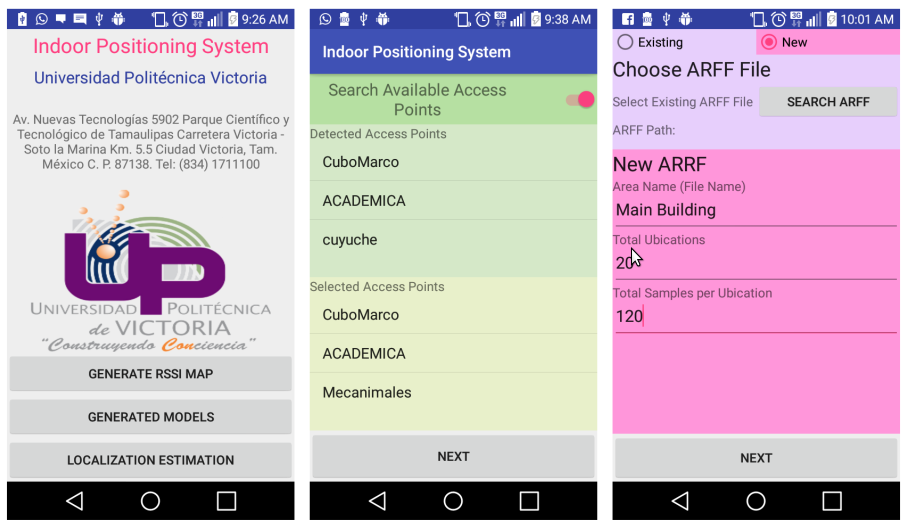
\includegraphics[width=0.75\textwidth]{Figs/IndoorPositionSystem3}
     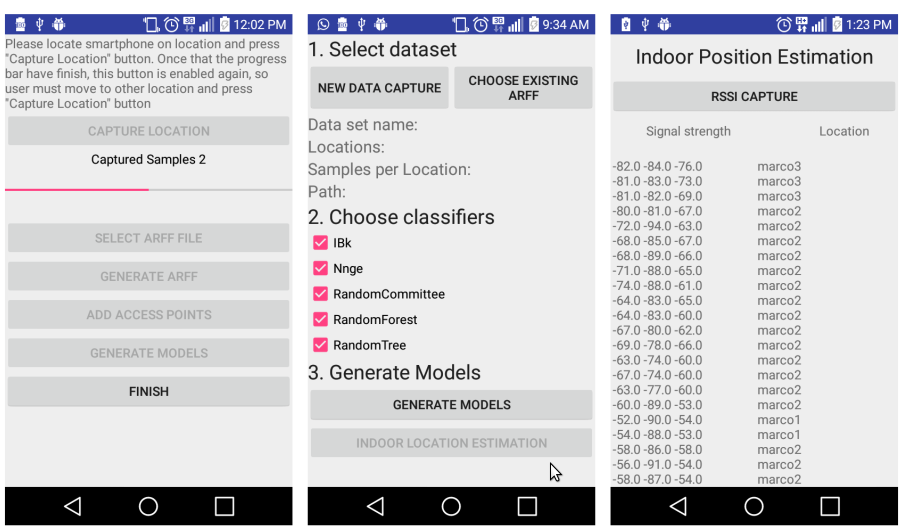
\includegraphics[width=0.75\textwidth]{Figs/IndoorPositionSystem4}
     \end{center}
\end{column}
\end{columns}
\end{block} 

\note[item]{\scriptsize In main screen of the App there are three main functionalities.} 
\note[item]{\scriptsize The first one allows the capture of RSSI data from the selected APs;}
\note[item]{\scriptsize The user is asked to select the access points required for
generating the RSSI map. Two list are displayed: the first one contains the available APs. As soon as the user selects an AP, this is stored in the second list.}
\note[item]{\scriptsize The app ask the user the number of locations, and the user must move along the desired locations and wait the app to capture a set of RSSI lectures for each location. This proccess is repeated until all the locations has been captured. }

\note[item]{\scriptsize The second one allows the user to train a model using data previously captured; }
\note[item]{\scriptsize The user selects the dataset to be used as the training file. In the second step, it is possible to select the models to be trained, and when the user presses the Generate Models button, the training starts.}

\note[item]{\scriptsize The third one allows the user to use previously generated models to get the current location.} %Each functionality is launched by a button located on
%the main screen}
%\note[item]{\scriptsize Once the training finishes, it is possible to estimate the real-time indoor localization, using data from previously-selected APs.}



\end{frame}

\begin{frame}{\citetitle{MarcoNuno_Revista_2018_07_00} (3)}
\begin{block}{Results} 
\begin{columns}
\begin{column}{0.7\textwidth}
\begin{itemize}
\item Data obtained from the proposed scenarios were used to train 59 different classifiers.
\item A two-fold cross-validation was utilized.
\item Mean accuracies of 100 executions of the top-12 classifiers are obtained.
\item The top-five selected classifiers are: NNge, Ibk, random tree, random forest and random committee.
\end{itemize}
\end{column}
\begin{column}{0.3\textwidth}  
    \begin{center}
     %%%%% this is a minipage, so \textwidth is already adjusted to the size of the column
     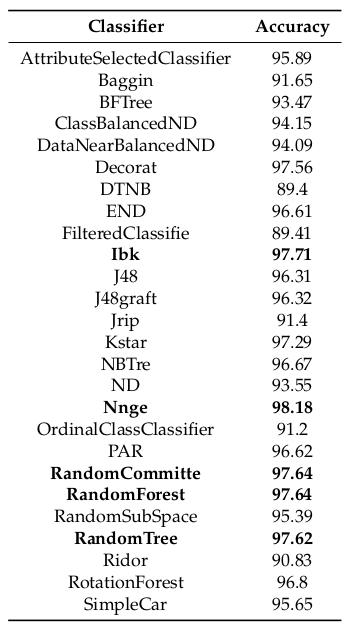
\includegraphics[width=0.6\textwidth]{Figs/IndoorPositionSystem5}
     \end{center}
\end{column}
\end{columns}

\note[item]{\scriptsize An off-line process was executed to determine which classifiers achieve higher accuracies}

\note[item]{\scriptsize 59 different classifiers were trained. For this purpose, a two-fold cross-validation was utilized, and the mean accuracies of 100 executions of the top-12 classifiers for the three dataset of the proposed scenarios were obtained}

\note[item]{\scriptsize For each location, a data capture process was performed using 3, 4 or 5 APs. From the results obtained, it can be concluded that increasing the number of APs is beneficial for most cases; however, in real scenarios,
it is not possible to add as many APs as needed.}

\end{block} 
\end{frame}


